\section*{24/06/2022 --- Pontos de Equilíbrio e Linearização}
\markboth{Pontos de Equilíbrio e Linearização}{24/06/2022}
\noindent\textbf{\sffamily Exercício 1.}
\begin{itemize}
	\item [a)] 
	Determine os pontos de equilíbrio do sistema abaixo.
	
	\item [b)] 
	Determine o sistema linearizado tangente de cada ponto de equilíbrio e analise sua instabilidade.
\end{itemize}
%
\[
\frac{d^2\theta}{dt^2} = 
\theta^2 - 2\theta - 10\frac{d\theta}{dt} 
\]
%

\noindent\textbf{\sffamily Exercício 2.}
\begin{itemize}
	\item [a)] 
	Determine os pontos de equilíbrio do sistema abaixo.
	
	\item [b)] 
	Determine o sistema linearizado tangente de cada ponto de equilíbrio e analise sua instabilidade.
\end{itemize}
%
\begin{align*}
	\frac{d\theta_1}{dt} &= 
	\theta_1^2 - 2\theta_2\theta_1 - u \\
	%
	\frac{d\theta_2}{dt} &= 
	\theta_1 -3\theta_2 + 2\sin\theta_2 + u\theta_2
\end{align*}
%
\rule{\textwidth}{0.5pt}


\noindent
\textbf{\sffamily Exercício 1 --- solução.}
\begin{itemize}
	\item [a)] 
	Primeiro definimos as equações de estado. 
	Pondo 
	$x_1 = \theta$ e 
	$x_2 = \dot{\theta}$, temos 
	%
	\begin{align*}
		\dot{x}_1 &= x_2 \\
		\dot{x}_2 &= x_1^2 - 2x_1 - 10x_2  
	\end{align*}
	%
	Seja $(\bar{x_1}, \bar{x_2})$ um ponto de equilíbrio. Por definição,
	%
	\begin{align*}
		\begin{array}{l}
			0 = \bar{x_2} \\
			0 = \bar{x_1}^2 - 2\bar{x_1} - 10\bar{x_2} 
		\end{array} 
		\quad\iff\quad 
		\bar{x_1} = 0 \text{ ou } \bar{x_1}=2, \quad 
		\bar{x_2} = 0.
	\end{align*}
	%
	Logo, os pontos de equilíbrio são 
	$P_1 = (0, 0)$ e 
	$P_2 = (2, 0)$.
	%		
	
	\item [b)] 
	Apenas a segunda equação de estado precisa ser linearizada 
	(como é possível tomar $y=x_1-\bar{x_1}$, a saída também não precisará ser linearizada).
	Temos 
	%
	\begin{align*}
		\dot{x}_2 = f_2(x_1, x_2) 
		&\approx f_2(\bar{x_1}, \bar{x_2}) 
		+
		\del_{x_1} f_2\bigg|_{\bar{x_1}, \bar{x_2}}
		(x_1 - \bar{x_1}) 
		+
		\del_{x_2} f_2\bigg|_{\bar{x_1}, \bar{x_2}}
		(x_2 - \bar{x_2}) \\
		&= (2\bar{x_1} - 2)(x_1 - \bar{x_1}) -
		10x_2,
	\end{align*}
	%
	e daí, pela mudança de variável 
	$x_1-\bar{x_1} \rightarrow x_1$, o sistema linearizado é  
	%
	\begin{align*}
		\begin{array}{l}
			\dot{x}_1 = x_2 \\
			\dot{x}_2 =(2\bar{x_1} - 2)(x_1 - \bar{x_1}) - 10x_2 
		\end{array}
		\quad \iff \quad 
		\begin{pmatrix}
			\dot{x}_1 \\ \dot{x}_2
		\end{pmatrix}
		&= 
		\begin{pmatrix}
			0 & 1 \\
			2\bar{x_1} - 2 & -10 
		\end{pmatrix}
		\begin{pmatrix}
			x_1 - \bar{x_1} \\ x_2 - \bar{x_2}
		\end{pmatrix},
		\\
		y&= \begin{pmatrix} 1 & 0 \end{pmatrix} 
		\begin{pmatrix} x_1 \\ x_2 \end{pmatrix}.
	\end{align*}
	%
	Considerando os valores dos pontos de equilíbrio, temos
	%
	\begin{align*}
		P_1 \implies 
		\dot{X} &= 
		\begin{pmatrix}
			0 & 1 \\
			- 2 & -10 
		\end{pmatrix}
		X, \\
		P_2 \implies 
		\dot{X} &= 
		\begin{pmatrix}
			0 & 1 \\
			2 & -10
		\end{pmatrix}
		\begin{pmatrix}
			x_1-2 \\ x_2
		\end{pmatrix}
	\end{align*}
	%
\end{itemize}
%

\clearpage
\noindent
\textbf{\sffamily Exercício 2 --- solução.}
\begin{itemize}
	\item [a)] 
	Seja $(\bar{\theta_1}, \bar{\theta_2})$ um ponto de equilíbrio. Então,
	%
	\[
	\begin{array}{l}
		0 = 
		\bar{\theta_1}^2 - 2\bar{\theta_2}\cdot \bar{\theta_1} - 0 \\
		%
		0 = 
		\bar{\theta_1} -3\bar{\theta_2} + 2\sin\bar{\theta_2} + 0
	\end{array}
	\implies
	\begin{array}{l}
		0 = 
		\bar{\theta_1}(\bar{\theta_1} - 2\bar{\theta_2}) \\
		%
		0 = 
		\bar{\theta_1} -3\bar{\theta_2} + 2\sin\bar{\theta_2}
	\end{array}.
	\]
	%
	Pela primeira equação acima, ou 
	$\bar{\theta_1}=0$ ou 
	$\bar{\theta_1} - 2\bar{\theta_2}=0$.
	Assumindo o primeiro caso, é imediato pela segunda equação que 
	$\sin\bar{\theta_2}=1,5\bar{\theta_2}$. 
	A série de Taylor do seno ao redor da origem nos diz que a única solução dessa equação é $\bar{\theta_2}=0$. 
	Por outro lado, assumindo $\bar{\theta_1}=2\bar{\theta_2}$, encontramos que 
	$\sin\bar{\theta_2} = 0,5\bar{\theta_2}$, que, novamente pela série de Taylor, possuirá 3 soluções. 
	Por auxílio de uma calculadora gráfica, as raízes são 
	$\bar{\theta_2} = 0$ (de novo),
	$\bar{\theta_2} \approx \pm 1,895$.
	Os pontos de equilíbrio ficam então 
	%
	\[
	P_1 = \begin{pmatrix} 0 \\ 0 \end{pmatrix}, \quad 
	P_2 = \begin{pmatrix} 3,79 \\ 1,895 \end{pmatrix}, \quad 
	P_3 = \begin{pmatrix} -3,79 \\ -1,895 \end{pmatrix}.
	\]
	%
	\begin{figure}[h!]\centering
		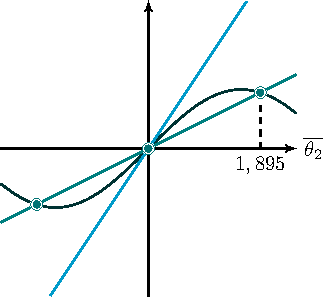
\includegraphics{em busca de theta2.pdf}
		\caption{%
			Gráficos em escala das funções $\sin\bar{\theta_2}$, 
			$0,5\bar{\theta_2}$, e
			$1,5\bar{\theta_2}$.
			Destaque para os pontos de interseção.
		}
	\end{figure}
	
	\item [b)] 
	Ambas equações de estado precisam ser linearizadas. 
	Temos 
	%
	\begin{align*}
		\dot{\theta}_1 = f_1(\theta_1, \theta_2; u)
		&\approx f_1(\bar{\theta_1}, \bar{\theta_2}; u) 
		+
		\del_{\theta_1} f_1
		\bigg|_{\bar{\theta_1}, \bar{\theta_2}}
		(\theta_1 - \bar{\theta_1}) 
		+
		\del_{\theta_2} f_1
		\bigg|_{\bar{\theta_1}, \bar{\theta_2}}
		(\theta_2 - \bar{\theta_2}) 
		+
		\del_{u} f_1
		\bigg|_{\bar{\theta_1}, \bar{\theta_2}}
		u 
		\\
		&= (2\bar{\theta_1} - 2\bar{\theta_2})(\theta_1 - \bar{\theta_1})
		-2\bar{\theta_2}(\theta_2 - \bar{\theta_2})
		-u, 
		\\
		\dot{\theta}_2 = f_2(\theta_1, \theta_2; u)
		&\approx f_2(\bar{\theta_1}, \bar{\theta_2}; u) 
		+
		\del_{\theta_1} f_2
		\bigg|_{\bar{\theta_1}, \bar{\theta_2}}
		(\theta_1 - \bar{\theta_1}) 
		+
		\del_{\theta_2} f_2
		\bigg|_{\bar{\theta_1}, \bar{\theta_2}}
		(\theta_2 - \bar{\theta_2}) 
		+
		\del_{u} f_2
		\bigg|_{\bar{\theta_1}, \bar{\theta_2}}
		u  
		\\
		&= (\theta_1 - \bar{\theta_1})+
		(-3-2\cos\bar{\theta_2})(\theta_2 - \bar{\theta_2})
		+\bar{\theta_2}u, 
	\end{align*}
	%
	e portanto
	%
	\[
	\begin{pmatrix}
		\dot{\theta}_1 \\ \dot{\theta}_2
	\end{pmatrix}
	= 
	\begin{pmatrix}
		2\bar{\theta_1} - 2\bar{\theta_2} & -2\bar{\theta_2} \\
		1 & -3+2\cos\bar{\theta_2} 
	\end{pmatrix}
	\begin{pmatrix}
		\theta_1 - \bar{\theta_1} \\ \theta_2 - \bar{\theta_2}
	\end{pmatrix}
	+
	\begin{pmatrix}
		-1 \\ \bar{\theta_2}
	\end{pmatrix},
	u
	\]
	%
	de forma que
	%
	\begin{align*}
		P_1 \implies \dot{\Theta} &= 
		\begin{pmatrix} 
			0 & 0 \\ 
			1 & -1
		\end{pmatrix}
		\Theta 
		+
		\begin{pmatrix} -1 \\ 0 \end{pmatrix} u, \\
		P_2 \implies \dot{\Theta} &=
		\begin{pmatrix} 
			3,79 & -7,58 \\ 
			1 & -1,001
		\end{pmatrix}
		\begin{pmatrix}
			\theta_1 - 3,79 \\
			\theta_2 - 1,895
		\end{pmatrix}
		+
		\begin{pmatrix} -1 \\ 1,895 \end{pmatrix} u, \\
		P_3 \implies \dot{\Theta} &=
		\begin{pmatrix} 
			-3,79 & 7,58 \\ 
			1 & -1,001
		\end{pmatrix}
		\begin{pmatrix}
			\theta_1 + 3,79 \\
			\theta_2 + 1,895
		\end{pmatrix}
		+
		\begin{pmatrix} -1 \\ -1,895 \end{pmatrix} u.
	\end{align*}
\end{itemize}
%